\Chapter{Párhuzamosítási lehetőségek}

\Section{Az OpenCL nyelv}

Open Computing Language egy keretrendszer amely lehetőséget ad olyan programok írására amelyek különböző platformokon is futtathatóak.
Az OpenCL meghatároz egy programozási nyelvet az eszközök és API-k számára a platformok vezérléséhez és a számítások végrehajtásához az eszközökön. Szabványos interfészt biztosít a párhuzamos számításokhoz, melyhez adatalapú és feladatalapú párhuzamosítást használ.

Fontos észrevenni, hogy az OpenCL natív módon képes beszélni az eszközök nagy részével, ez nem azt jelenti, hogy a kód optimálisan fog futni. Ugyanis különböző Cl eszközök különböző funkciókkal vannak ellátva. Gyártó specifikus kiterjesztések elkerülésével a kód hordozható lesz, de nem sebesség optimális.

\begin{figure}[h!]
\centering
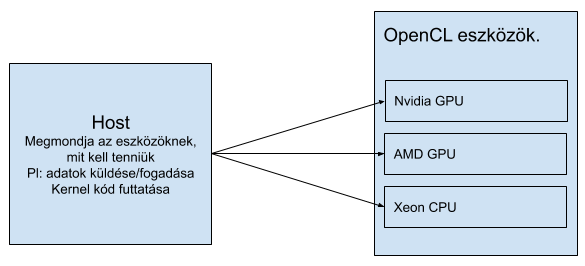
\includegraphics[width=\textwidth]{images/opencl.png}
\caption{OpenCL}
\label{fig:opencl}
\end{figure}

A következő esetekben a GPU-t érdemes használni.
\begin{itemize}
\item Gyors permutáció: Az eszközök gyorsabban mozgatáják a memóriát mint a Host.
\item Adat átváltás: Egyik formátumról másikra.
\item Numerikus gyorsítás: Az eszközök gyorsabban számolnak nagyobb adatdarabokkal mint a Host.
\end{itemize}
Jelen esetben a Host egy asztali számítógép.
Számítási eszközei: CPU, GPU, FPGA, DSP.
A számítási egységek: a magok száma
Elemek feldolgozása: ALU-k magunként.

OpenCL használata mellett szükségtelen gondolkozni azon, hogy pontosan mi is végzi el a számításokat. Ugyanis az OpenCL modelljének illeszkedése egy adott hardverhez, a gyártók feladata.
